\section{Evaluation}
\label{sec.evaluation}
To demonstrate that our popular paths based approach is practical as well as effective in improving container security, 
we conducted a series of tests to answer the following questions: 
\begin{itemize}
	\item Can we obtain the popular paths data for containers in a systematic way? (Section~{\ref{sec.evaluation.1}})
	\item Can an analysis of the popular paths data for containers help developers and researchers achieve better security? (Section~{\ref{sec.evaluation.2}})
	\item Can real-world containers run only on the popular paths with no loss of functionality? (Section~{\ref{sec.evaluation.3}})
	\item What is the performance overhead of using UnPAK, as opposed to using the original Linux kernel? (Section~{\ref{sec.evaluation.4}})
	\item How does this work compare against current kernel tailoring methods in reducing the attack surface? (Section~{\ref{sec.evaluation.5}})
\end{itemize}

\subsection{Can popular paths data for containers be collected in a systematic way?}
\label{sec.evaluation.1} 
Having a systematic way to obtain the popular paths data for containers is key to making its use scalable, reproducible, and accessible to developers and the research community. 
Therefore, the first step in our investigation was developing and testing such a standard procedure for containers. 
This procedure can be divided into three stages: selecting the \textbf{dataset}, assembling \textbf{a profiling framework}, and conducting the \textbf{experiment}. 

\textbf{The dataset:} The dataset stage involved selecting the containers to use and the workload that would run inside of them. 
We wanted the defined dataset to be representative of the containers used by millions of clients, so we sourced a set accepted as widely used according to trustworthy real-world statistics. 
We selected 50 containers deemed most popular on Docker Hub according to its official number of pulls. Each selected container had more than 10 million pulls \cite{DockerHub}. 
The workload run by each was the set of commands or operations defined in the official Dockerfile for each container image. 

\textbf{The profiling framework:} This next stage involved establishing a running environment and capturing the actual data. 
The procedure required a robust framework, and ideally we wanted it to be portable so it could be used across different platforms. We selected the LinuxKit VM, 
which works with Linux, Windows, and Mac OS, and a Linux kernel with a Gcov profiling tool enabled to run the Docker containers. 
This framework works with  other Linux kernel versions, which makes the procedure more widely applicable. 

\textbf{The experiment:} The test itself consisted of running the containers from the dataset with their defined workloads in the profiling framework, and extracting the resulting data. 
The procedure automated the experimental runs in a way that allowed users to define key variables of the input, such as the exact version of the container image to use, 
and the number of iterations to run for each container. This design choice makes our procedure flexible, and better able to accommodate users with different needs 
and computing resources. In our experiment, we decided to do 10 iterations, 
because it provides a sufficient number of runs to make the data reliable while not consuming too much time and computing resources. 

\subsection{What security benefits can be obtained from using the popular paths data?}
\label{sec.evaluation.2} 
Using the procedures described above, we obtained data for some of the most frequently accessed  containers on Docker Hub, and used it to check  for security vulnerabilities. 
We started with a list of all 50 of the CVE kernel vulnerabilities for Linux kernel version 4.14.x that were available from the National Vulnerability Database 
when our study was conducted (July 2019) \cite{NVD} and identified the kernel patch that fixed the bug. 
This allowed us to identify the source line numbers, functions and files that corresponded to it, and use this information to highlight where these bugs were located in the kernel.  

It should be noted that 49 out of the 50 bugs tested in this experiment were discovered and confirmed after publication of the original popular paths study \cite{Lock-in-Pop}. 
This shows that the metric can indeed effectively predict where bugs are likely to occur. 

The raw data generated by Gcov in our profiling framework was at the line-of-code level, as this is the level at which our initial popular path study was done. 
We then processed it to generate  additional information at the function and file level. 
These three different levels of granularity provide a full map of how the kernel code was used by containers and where the vulnerabilities might lie in each.

\noindent
\textbf{Popular paths data at the file level}
\newline
For developers and security teams, the first thing to identify is which files are popular, 
as this can be a first step to secure the kernel without needing to deal with the complex logic and branches inside of each file. 
We deemed a file as ``popular'' if any line of code inside of it was in the raw popular paths data we obtained. 

From our data (shown in Table \ref{tab:cve_files}), we can see that the all-popular files, or files in which every line is popular, contain no bugs  and thus are the safest ones to use. 
Alternatively, the unpopular files contain more than half of the bugs. 
The higher bug density of the unpopular files suggests that removing these files could be an easy first step to securing the kernel. 

The files designated as ``partially popular,'' which accounted for about 30\% of the bugs investigated, present a trickier problem to resolve. 
The presence of some popular lines means these items are being used and can not simply be removed. If stricter security requirements are desired, 
we need to go inside of these files to look at a finer granularity, which is the function level. 

\begin{table}
\caption{CVE bugs located in Unpopular and Popular kernel files}
\label{tab:cve_files}
\begin{tabular}{l|r|r|r|r|r}
 kernel & unpop & pop & all-pop & partial-pop & total \\
 dir & \color{red}{(CVEs)} & \color{red}{(CVEs)} & \color{red}{(CVEs)} & \color{red}{(CVEs)} & \\
 \hline
 arch & 133\color{red}{(3)} & 272\color{red}{(1)} & 81 & 191\color{red}{(1)} & 405 \\
 \hline
 block & 10 & 44 & 0 & 44 & 54 \\
 \hline
 crypto & 53\color{red}{(1)} & 89\color{red}{(2)} & 0 & 89\color{red}{(2)} & 142 \\
 \hline
 drivers & 161\color{red}{(11)} & 543\color{red}{(3)} & 5 & 538\color{red}{(3)} & 704 \\
 \hline
 fs & 52\color{red}{(6)} & 176\color{red}{(2)} & 5 & 171\color{red}{(2)} & 228 \\
 \hline
 ipc & 1 & 9 & 0 & 9 & 10 \\
 \hline
 kernel & 40\color{red}{(2)} & 183 & 2 & 181 & 223 \\
 \hline
 mm & 16\color{red}{(1)} & 59\color{red}{(4)} & 0 & 59\color{red}{(4)} & 75 \\
 \hline
 net & 266\color{red}{(5)} & 482\color{red}{(3)} & 0 & 482\color{red}{(3)} & 748 \\
 \hline
 security & 6 & 17 & 0 & 17 & 23 \\
 \hline
 total & 738\color{red}{(29)} & 1874\color{red}{(15)} & 93 & 1781\color{red}{(15)} & 2612 \\
 \hline 
 percent & 28.3\% & 71.7\% & 3.6\% & 68.1\% & 100\% \\
 & \color{red}{(66\%)} & \color{red}{(34\%)} & \color{red}{(0\%)} & \color{red}{(34\%)} &
\end{tabular}
\textit{\textbf{unpop}: contain 0 line of popular code.} \\
\textit{\textbf{all-pop}: every line is popular code.} \\
\textit{\textbf{partial-pop}: contain at least 1 line of popular code and 1 line of unpopular code.} \\
\textit{\textbf{pop}: all-pop + partial-pop.}
\end{table}

\noindent
\textbf{Popular paths data at the function level}
\newline
Using the raw data, shown in Table \ref{tab:cve_functions}, we pinpoint which file functions were used by popular containers. 
Our data shows that functions deemed unpopular contain 5x more bugs than popular functions, 
while the all-popular functions (every line in the function is  popular) contain only one bug. 

As with the file analysis above, having this information can help security teams eliminate some risks by just avoiding the less-used functions. 
Unfortunately, that still leaves the partially-popular functions, which  contain 12 bugs.  As with the partially-popular  files, 
the presence of some frequently used functions in this group means they cannot  simply be removed at this level. 
While analyzing each function at the line-of-code level is the most labor intensive of the methods elaborated here, 
it offers the best opportunity to remove risky code. Below we look at vulnerabilities revealed by the popular paths data at this most fine-grained level. 

\begin{table}
\caption{CVE bugs located in Unpopular and Popular kernel functions}
\label{tab:cve_functions}
\begin{tabular}{l|r|r|r|r|r}
 kernel & unpop & pop & all-pop & partial-pop & total \\
 dir & \color{red}{(CVEs)} & \color{red}{(CVEs)} & \color{red}{(CVEs)} & \color{red}{(CVEs)} & \\
 \hline
 arch & 1528\color{red}{(7)} & 968\color{red}{(1)} & 312 & 656\color{red}{(1)} & 2496 \\
 \hline
 block & 777 & 264 & 68 & 196 & 1041 \\
 \hline
 crypto & 527\color{red}{(6)} & 121 & 36 & 85 & 648 \\
 \hline
 drivers & 6258\color{red}{(20)} & 2640 & 562 & 2078 & 8898 \\
 \hline
 fs & 1888\color{red}{(13)} & 1653\color{red}{(3)} & 559 & 1094\color{red}{(3)} & 3541 \\
 \hline
 ipc & 138 & 102 & 33 & 69 & 240 \\
 \hline
 kernel & 3562\color{red}{(8)} & 2280 & 793 & 1487 & 5842 \\
 \hline
 mm & 976\color{red}{(2)} & 889\color{red}{(6)} & 281 & 608\color{red}{(6)} & 1865 \\
 \hline
 net & 3703\color{red}{(9)} & 2405\color{red}{(3)} & 695\color{red}{(1)} & 1710\color{red}{(2)} & 6108 \\
 \hline
 security & 179 & 201 & 104 & 97 & 380 \\
 \hline
 total & 19536\color{red}{(65)} & 11523\color{red}{(13)} & 3443\color{red}{(1)} & 8080\color{red}{(12)} & 31059 \\
 \hline 
 percent & 62.9\% & 37.1\% & 11.1\% & 26\% & 100\% \\
 & \color{red}{(83.3\%)} & \color{red}{(16.7\%)} & \color{red}{(1.3\%)} & \color{red}{(15.4\%)} &
\end{tabular}
\end{table}

\begin{table*}
  \begin{center}
    \caption{Evaluation of the CVE vulnerabilities at the line level}
    \label{tab:evaluation_cve}
    \begin{tabular}{c|l|c|c|c} % <-- Alignments: 1st column left, 2nd middle and 3rd right, with vertical lines in between
      \textbf{\#} & \textbf{CVE ID} & \textbf{CVSS Score} & \textbf{Description} & \textbf{Detected in the}\\
       & & & & \textbf{LinuxKit Popular Paths}\\
      \hline
      1 & CVE-2019-10124 & 7.8 & denial of service, in mm/memory-failure.c & \ding{55}\\
      2 & CVE-2019-9213 & 4.9 & kernel NULL pointer dereferences, in mm/mmap.c & \ding{55}\\
      3 & CVE-2019-9003 & 7.8 & use-after-free & \ding{55}\\
      4 & CVE-2019-8956 & 7.2 & use-after-free & \ding{55}\\
      5 & CVE-2019-8912 & 7.2 & use-after-free & \ding{55}\\
      6 & CVE-2019-7308 & 7.5 & out-of-bounds speculation on pointer arithmetic & \ding{55}\\
      7 & CVE-2019-3701 & 7.1& privilege escalation & \ding{55}\\
      8 & CVE-2018-1000204 & 6.3 & copy kernel heap pages to the userspace & \ding{55}\\
      9 & CVE-2018-1000200 & 4.9 & NULL pointer dereference & \ding{55}\\
      10 & CVE-2018-1000026 & 6.8 & denial of service & \ding{55}\\
      11 & CVE-2018-20511 & 2.1 & privilege escalation & \ding{55}\\
      12 & CVE-2018-20169 & 7.2 & mishandle size checks & \ding{55}\\
      13 & CVE-2018-18690 & 4.9 & unchecked error condition & \ding{55}\\
      14 & CVE-2018-18445 & 7.2 & out-of-bounds memory access & \ding{55}\\
      15 & CVE-2018-18281 & 4.6 & improperly flush TLB before releasing pages & \ding{55}\\
      16 & CVE-2018-18021 & 3.6 & denial of service & \ding{55}\\
      17 & CVE-2018-16862 & 2.1 & the cleancache subsystem incorrectly clears an inode & \ding{55}\\
      18 & CVE-2018-16658 & 3.6 & local attackers could read kernel memory & \ding{55}\\
      19 & CVE-2018-16276 & 7.2 & privilege escalation & \ding{55}\\
      \color{red}{20} & \color{red}{CVE-2018-15594} & \color{red}{2.1} & \color{red}{spectre-v2 attacks against paravirtual guests} & \color{red}{\ding{51}}\\
      \color{red}{21} & \color{red}{CVE-2018-15572} & \color{red}{2.1} & \color{red}{userspace-userspace spectreRSB attacks} & \color{red}{\ding{51}}\\
      22 & CVE-2018-14646 & 4.9 & NULL pointer dereference & \ding{55}\\
      23 & CVE-2018-14634 & 7.2 & integer overflow, privilege escalation & \ding{55}\\
      24 & CVE-2018-14633 & 8.3 & stack buffer overflow & \ding{55}\\
      25 & CVE-2018-14619 & 7.2 & privilege escalation & \ding{55}\\
      26 & CVE-2018-13406 & 7.2 & integer overflow & \ding{55}\\
      27 & CVE-2018-12904 & 4.4 & privilege escalation & \ding{55}\\
      28 & CVE-2018-11508 & 2.1 & local user could access kernel memory & \ding{55}\\
      29 & CVE-2018-11412 & 4.3 & ext4 incorrectly allows external inodes for inline data & \ding{55}\\
      30 & CVE-2018-10940 & 4.9 & incorrect bounds check allows kernel memory access & \ding{55}\\
      31 & CVE-2018-10881 & 4.9 & denial of service & \ding{55}\\
      32 & CVE-2018-10880 & 7.1 & denial of service & \ding{55}\\
      33 & CVE-2018-10879 & 6.1 & use-after-free & \ding{55}\\
      34 & CVE-2018-10878 & 6.1 & denial of service & \ding{55}\\
      35 & CVE-2018-10074 & 4.9 & denial of service & \ding{55}\\
      36 & CVE-2018-10021 & 4.9 & denial of service & \ding{55}\\
      37 & CVE-2018-8781 & 7.2 & code execution in kernel space & \ding{55}\\
      38 & CVE-2018-6555 & 7.2 & denial of service & \ding{55}\\
      39 & CVE-2018-6554 & 4.9 & denial of service & \ding{55}\\
      40 & CVE-2018-5390 & 7.8 & denial of service & \ding{55}\\
      41 & CVE-2018-1130 & 4.9 & NULL pointer dereference & \ding{55}\\
      \color{red}{42} & \color{red}{CVE-2018-1120} & \color{red}{3.5} & \color{red}{denial of service} & \color{red}{\ding{51}}\\
      43 & CVE-2018-1118 & 2.1 & kernel memory leakage & \ding{55}\\
      44 & CVE-2018-1068 & 7.2 & write to kernel memory & \ding{55}\\
      45 & CVE-2017-1000410 & 5.0 & leaking data in kernel address space & \ding{55}\\
      46 & CVE-2017-1000407 & 6.1 & denial of service & \ding{55}\\
      47 & CVE-2017-1000405 & 6.9 & overwrite read-only huge pages & \ding{55}\\
      48 & CVE-2017-18224 & 1.9 & race condition, denial of service & \ding{55}\\
      49 & CVE-2017-18216 & 2.1 & NULL pointer dereference, denial of service & \ding{55}\\
      50 & CVE-2015-5327 & 4.0 & out-of-bounds memory read & \ding{55}\\
    \end{tabular}
  \end{center}
\end{table*}

\noindent
\textbf{Popular paths data at the line level}
\newline
An analysis of the gathered data at the line level shows that the popular lines make up about  20\% of the kernel codebase, 
and that only 6\% (or three) of the CVE bugs were detected in those lines (Table \ref{tab:evaluation_cve}.) 
These three bugs were in commonly used kernel code that, to the best of our knowledge, 
cannot be avoided by any existing security systems. We describe these three bugs in more detail below.  

It is important, to note, however, that two of these bugs  (CVE-2018-15594 and CVE-2018-15572) are Spectre-related hardware vulnerabilities, 
based on fundamental flaws in CPU’s data cache and speculative execution. 
These flaws affect many modern processors [69], and software tools and compartmentalization techniques are not designed to prevent them. 
The only software-related bug is  CVE-2018-1120, which is related to the \texttt{mmap()} system call, and regularly accessed by virtualization systems. 

\noindent
\textbf{[CVE-2018-15594]} 
\newline
This bug lies in \texttt{arch/x86/kernel/paravirt.c} in the Linux kernel before 4.18.1. The source code mishandles certain indirect calls, 
making it easier for attackers to conduct Spectre-v2 attacks against paravirtual guests. 
In our tests, this bug was found in the  kernel trace data, and was reached frequently by programs running in LinuxKit. 
This occurs because the code inside of the \texttt{paravirt\_patch\_call()} function in \texttt{arch/x86/kernel/paravirt.c} is used to rewrite an indirect call with a direct call, 
an essential function used to support Linux kernel paravirtualization.

\noindent
\textbf{[CVE-2018-15572]} 
\newline
The \texttt{spectre\_v2\_select\_mitigation function} in \\
\texttt{arch/x86/kernel/cpu/bugs.c} in the Linux kernel before 4.18.1 does not always fill RSB upon a context switch. 
This makes it easier for attackers to conduct userspace-userspace spectreRSB attacks. 
As this piece of code in the \\
\texttt{spectre\_v2\_select\_mitigation(void)} function would be used by every program as the kernel attempts to mitigate potential Spectre attacks, 
it explains why it appeared in our LinuxKit popular paths. 

\noindent
\textbf{[CVE-2018-1120]} 
\newline
This vulnerability was found affecting the Linux kernel before version 4.17. 
by \texttt{mmap()ing} a FUSE-backed file onto the memory of a process containing command line arguments (or environment strings). 
It appears in the popular paths because \texttt{mmap()} is a commonly used system call. 
Furthermore, this vulnerability involves \texttt{proc\_pid\_cmdline\_read()} and \texttt{environ\_read()} functions  that are commonly invoked by virtual machines and user programs. 
According to CVSS 3.0 \cite{CVSS} metrics, this bug has ``high'' attack complexity, suggesting that it is very hard to exploit it in practice. 
Therefore, the negative impact of this bug’s existence is low. 

While a potential user of the popular paths metric must be aware of these bugs, 
limiting the risks to just these three greatly reduces the odds of having to deal with repeated and costly incidents from zero-day vulnerabilities. 
In addition, the actions instrumented into UnPAK were able to catch any attempt to reach these bugs, giving users alerts and options to terminate or block the risky programs trying to trigger the bugs. 

An important result of this multi-level data analysis, was the discovery that users actually had a hierarchy of security choices, rather than one ``all or nothing'' option. 
Based on the sensitivity of the application and the resources available, users can actually choose the appropriate tradeoff of effort vs.security appropriate for them. 
File level information helps identify unused portions of the kernel at a glance, and can eliminate a large number of kernel vulnerabilities in a quick first step, 
with little expenditure of time and effort. The function level information enlarges the scope by focusing on less-used functions and suggesting the value of eliminating the bugs inside these functions. 
Less security sensitive applications could consider stopping at either one of these first two levels. 
But, for those applications where security is critical, moving on to the line level will give the most accurate information about where bugs are located and the most precise instructions for modifying the kernel.

\noindent
\textbf{Are there sufficient commonalities across different containers to form a valid dataset for the most frequently used  containers? } 
\newline
To ensure our findings could be applicable to a broad variety of containers, we needed to establish that the data we found shared  common ground in their kernel footprints. 
Were there enough commonalities to form a realistic popular paths dataset to support multiple popular containers in real practice? 
If so, we could use  the kernel trace, or the record of all kernel code executed, from just a sample of containers to represent the trace of many more. 

To answer this question, we used the CDF (Cumulative Distribution Function) to analyze how soon the kernel trace of different containers would converge. 
Results of the CDF, as visualized in Figure \ref{fig:pp-cdf}, point out that the trace of the top six popular containers covered about 98\% of the total kernel trace for 25 containers. 
This offers additional corroboration that the popular paths data we collected is valid not only for the few containers we ran, but also for hundreds of containers on Docker Hub.  

\begin{figure*}
\centering
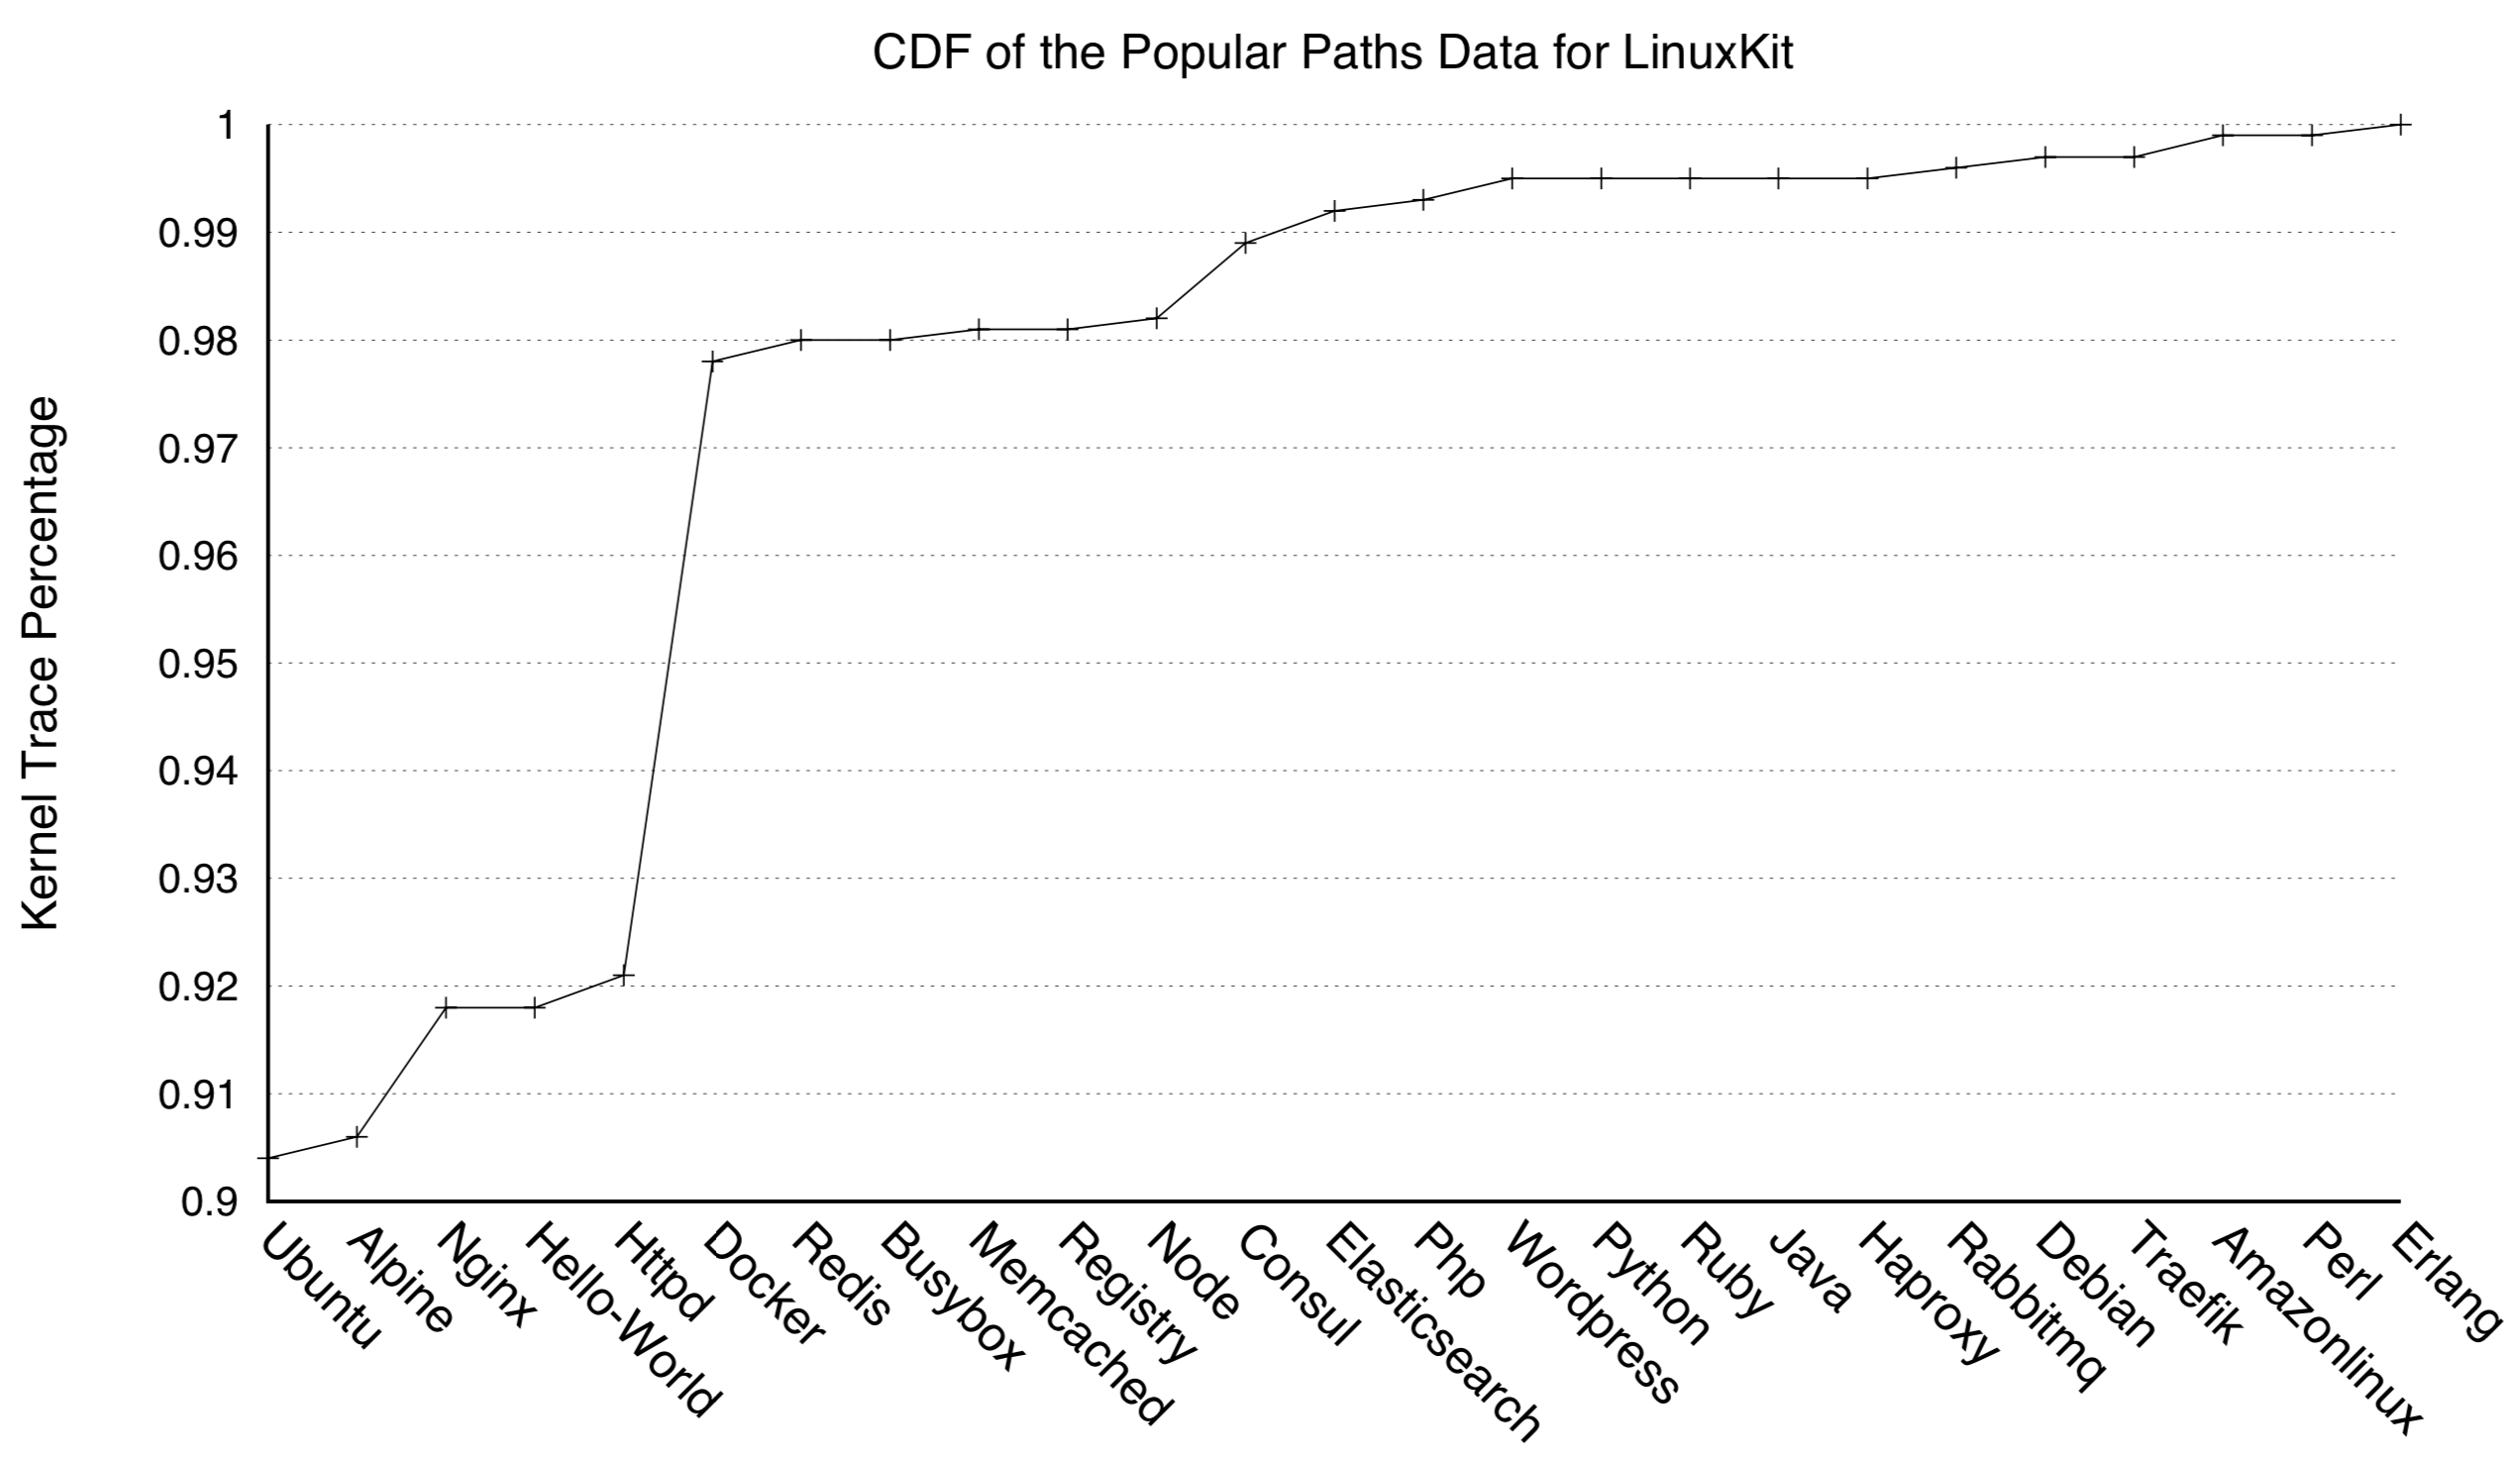
\includegraphics[width=1.5\columnwidth]{diagram/pp-cdf.png}
\caption{\small CDF of the popular paths of Docker containers showing most share the same kernel footprint}
\label{fig:pp-cdf}
\end{figure*}

In addition to the always used popular paths, which we identified as the common kernel lines that appeared each and every time, 
we also discovered certain lines of kernel code that showed up sporadically. 
For these lines, we looked at what activities they performed, and how common they were across different containers. 
In our analysis of the kernel trace of 10 frequently used Docker containers, we identified eight pieces of infrequently executed kernel code common among them. 
These traces are presented graphically in Figure \ref{fig:cdf-marked}. 
\begin{enumerate}
	\item \verb|kernel/cgroup/freezer.c|: a cgroup is freezing if any FREEZING flags are set.
	\item \verb|kernel/locking/rwsem-xadd.c|: waiting for a write lock to be granted. 
	\item \verb|kernel/locking/rwsem-xadd.c|: waiting for the read lock to be granted.
	\item \verb|mm/filemap.c|: process waitqueue for pages and check for a page match to prevent potential waitqueue hash collision. 
	\item \verb|fs/exec.c|: all other threads have exited, wait for the thread group leader to become inactive and to assume its PID. 
	\item \verb|kernel/workqueue|: insert a barrier work in the queue. According to the comments from the kernel source code, 
	the reason for inserting a barrier work seems to be to prevent a cancellation. 
	This is because \\
	\verb|try_to_grab_pending()| can not determine whether the work to be grabbed is at the head of the queue and thus can not clear LINKED flag of the previous work. 
	There must be a valid next work after a work with a LINKED flag set. 
	\item \verb|arch/x86/kernel/tsc.c|: try to calibrate the TSC \\ 
	against the Programmable Interrupt Timer and return the frequency of the TSC in kHz. 
	\item \verb|kernel/locking/mutex.c|: hand off a mutex. Give up ownership to a specific task, when @task = NULL, this is equivalent to a regular unlock.
\end{enumerate}

\begin{figure*}
\centering
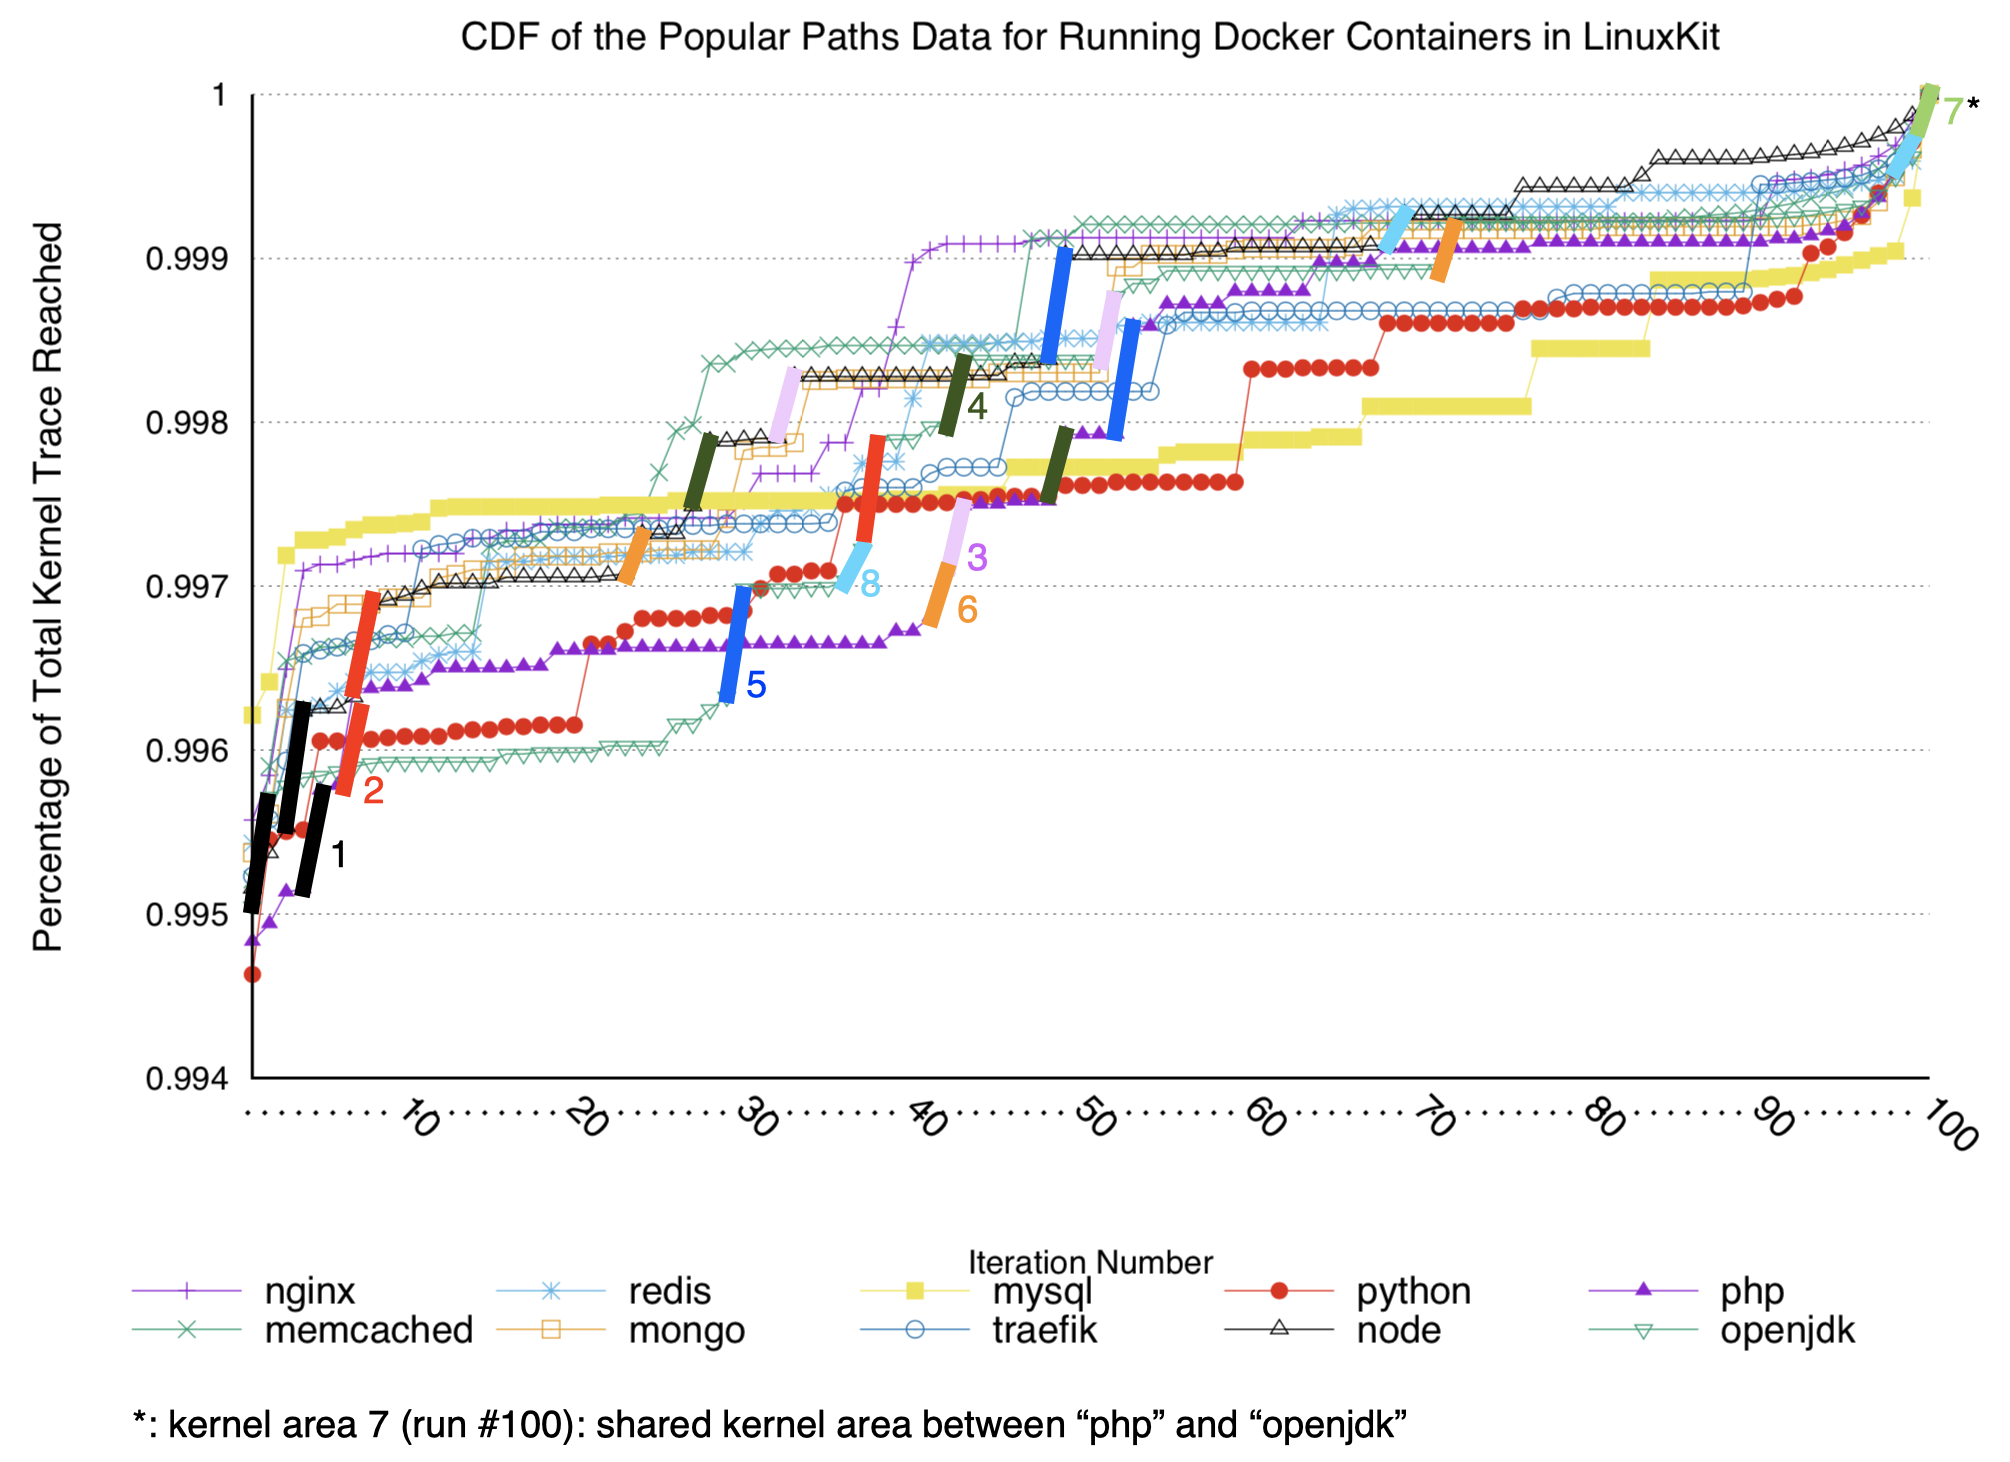
\includegraphics[width=1.5\columnwidth]{diagram/cdf-marked.png}
\caption{\small Common kernel code identified across different containers}
\label{fig:cdf-marked}
\end{figure*}

What this analysis tells us is that, despite the fact that they are infrequently executed, this code performs essential kernel functions and is used by multiple containers. 
Therefore, they should still be considered popular paths. On closer examination, we learn they are not always executed during each run because, as race-condition related codes, 
they depend on locks, and system conditions that may vary during different runs. 
Being able to capture these examples of infrequently-executed code and include them into our popular paths data is important, because it makes our UnPAK more reliable. 

\subsection{Can real-world containers run only on the popular paths with no loss of functionality?}
\label{sec.evaluation.3} 
Based on the popular paths data,  UnPAK can initiate multiple types of actions to enhance container security. 
While our initial tests documented here focused just on logging and warning, UnPAK actions could also include kernel panic, VM (Virtual Machine) exit, and code removal.  
Each of these actions has its own pros and cons. In this section we first present the results of functionality tests on UnPAK’s current instantiation, 
and then discuss alternative actions, and how they might affect operations

\subsubsection{Functionality evaluation of UnPAK with logging and warning actions}
\label{sec.evaluation.3.1} 
The next set of tests were to determine if  running applications in UnPAK, as currently instantiated, will cause any loss of functionality, as compared to using the original Linux kernel. 
The first study used the Linux Testing Project (LTP) \cite{LTP} test suites—an open source test project designed to validate the reliability, robustness, and stability of Linux—
to verify that  UnPAK functions as anticipated. The second test involved running a collection of the most popular containers from Docker Hub to verify if they were able to function correctly if they accessed only the popular paths.

\noindent
\textbf{Testing functionality with the LTP test suites} 
\newline
\textbf{Experimental Setup:} We used the Dockerfile provided by LinuxKit \cite{LinuxKit} to create the container image that runs the LTP version 20170116. 
This test project offers a set of regression and conformance tests designed to let members of the open source community confirm behavior of the Linux kernel. 
The test script we ran consisted of 798 test cases that verified the correctness of system functionalities, such as memory allocation, network connection, file system access, locking, and more. Using the test suites, we ran our experiments inside of a LinuxKit version 0.2+ virtual machine. 
The machine was built using Docker version 18.03.0-ce running on a host operating system of Ubuntu 16.04 LTS, with Linux kernel 4.13.0-36-generic. 
A QEMU emulator version 2.5.0 served as the local hypervisor. 

\textbf{Results:} UnPAK was able to run all of the 798 test cases, and as shown in Table \ref{tab:evaluation_ltp_results}, produced the same results as the original unmodified Linux kernel. 
Among all these tests, 673 of them generated “success” as their expected output on both kernels. We observed 105 test cases returned ``failures'' as expected, 
mainly because of restrictions imposed by LinuxKit. For example, \texttt{mem01} test failed because the malloc function failed to allocate 3056 MB memory due to the default memory restriction; 
the \texttt{gf01} test failed due to ``no space left on device'' in LinuxKit. the \texttt{swapon01} test failed due to swapfile not available, and more. 
There were 20 tests skipped due to certain required functions being unavailable in the LinuxKit VM version we tested. For example, the swap file was not accessible in LinuxKit, 
therefore the related \texttt{swapoff} test iterations were skipped intentionally.

\begin{table}
\begin{center}
\caption{LTP test results}
\label{tab:evaluation_ltp_results}
\begin{tabular}{c|c|c}
 & Original Linux kernel & UnPAK \\
 \hline
 Expected Success & 673 & 673 \\
 \hline
 Expected Failures & 105 & 105 \\
 \hline
 Skipped & 20 & 20 \\
 \hline
 Total & 798 & 798 \\ 
\end{tabular}
\end{center}
\end{table}

In summary, UnPAK yields the exact same output as the unmodified Linux kernel when running the 798 test cases in the LTP test suites. 
This shows that our logging implementation, using kvm hypercalls, can guarantee functionality correctness. 
It should be noted that a naive approach of logging using the kernel's \texttt{printk()} function did not work properly, 
because loops in some test cases will invoke a large number of \texttt{printk()} calls and result in a time-out error. 
For example, the \texttt{msgctl08} test case would invoke massive repeated \texttt{printk()} calls inside \texttt{ipc/util.c} and \texttt{ipc/msg.c} files. 
In addition to providing the correct functionality, UnPAK was able to capture and record all the unpopular paths accessed by the LTP test suites. 
This provides data that can help users understand the kernel footprint of different test cases. 

\noindent
\textbf{Testing functionality on real-world container applications} 
\newline
\textbf{Experimental Setup:} To confirm that UnPAK could run applications in real-world practice, we identified the 100 most downloaded containers from Docker Hub, 
and ran them in the same version of the LinuxKit virtual machine used in the test described in 4.3.1. 
Each container was run in the LinuxKit VM using the commands from its official Docker image. 
To take into account any potential variances, each container was run 10 times in the exact same environment.

\textbf{Results:} We verified that the 100 containers run using UnPAK were able to finish their normal workloads with, on average, less than 1\% of runtime overhead. 
In doing so, the containers used less than 0.1\% of the unpopular paths. As this data proves real-world containers can run on only the popular paths in most (>99.9\%) cases, 
it strongly argues the feasibility of creating a popular-paths based host kernel to run Docker containers.  

\subsubsection{Discussion on alternative actions}
\label{sec.evaluation.3.2} 
We  implemented a version of UnPAK with logging and warning capabilities as one instance of the type of actions this tailored kernel could perform. 
While we established in this study that logging and generating security warnings via UnPAK worked with real-world containers, 
we believe the kernel could  be instrumented to take other actions to improve security. 
In this section, we discuss three alternative actions for UnPAK: kernel panic, VM (Virtual Machine) exit, and code removal. 

Inserting the kernel \texttt{panic()} function in front of each unpopular code block could prevent containers from triggering zero-day bugs in the risky unpopular paths. 
In this modification, whenever a container attempts to reach unpopular paths, the host kernel will ``panic'' and stop the execution. 
We tried out this strategy and found it was not ideal. We tried adding \texttt{panic()} calls at locations related to existing CVE bugs, 
and verified that the kernel did successfully prevent the bug from being triggered. However, adding a \texttt{panic()} call to every unpopular path will incorrectly render the kernel function. 
Some kernel code under \texttt{init/} directory is  required during the boot stage, and cannot be modified with \texttt{panic()} calls. 
In addition, the kernel code needed by the \texttt{panic()} call itself cannot be instrumented without  breaking the function. 
As causing the host kernel to panic is not an elegant way to end programs, and may not be suitable for many users, this strategy is not a practical solution. 

A better way to stop code execution on risky unpopular paths is to invoke a VM exit, since this gives users more control over what to do next and avoids a kernel crash. 
With our current UnPAK implementation, we can directly deploy the VM exit action if desired. 
With the kernel logs provided by UnPAK, we can simply run a script from the host to monitor and check if there is any log entry showing an attempt to reach unpopular paths. 
If so, the script just needs to issue a command to let the LinuxKit VM shutdown. 
The disadvantage with this is that we would have to shut down the entire VM and every container running inside. 
If there are multiple containers running at the same time and only one of them exhibits suspicious behavior, 
we do not at this time have a reliable way to figure out which container was trying to reach the unpopular paths. 
But, it may be possible to infer that information from the memory. This would require a bit more effort, but  would be an interesting future work project.

Lastly, removing code on unpopular paths would be the most direct action, but this solution lacks flexibility. 
One possible action is to remove all the unpopular paths from the source code, which could cause trouble if some of it was needed by specific programs or 
in rare situations the kernel has to handle. Some unpopular code may also be needed by kernel internal functions, so it might not be a good idea to simply remove it. 
We have not implemented this action yet, but are interested in exploring it to see how well it works. 

\subsection{Performance Evaluation}
\label{sec.evaluation.4} 
Adoption of UnPAK is dependent on its real-world viability. So, the next round of tests were to ensure it would not negatively affect performance overhead costs. 
To demonstrate this, we evaluated both the run-time performance and memory space overhead of the modified kernel.

\textbf{Experimental Setup:} We compared data from containers running on the original Linux kernel and on the popular-paths based kernel and measured the overhead costs. 
We used the exact same running environment and configuration to ensure a fair comparison. In each test, the container finished its workload as defined in the official Dockerfile. 
We then measured the runtimes for both kernels and compared them. 

\textbf{Results:} On average, the results show running containers on UnPAK incurred about 0.5\% to 1\% of extra performance overhead, as compared to the original kernel. 
Results of the top 10 containers are shown in Figure \ref{fig:performance}.

\begin{figure*}
\centering
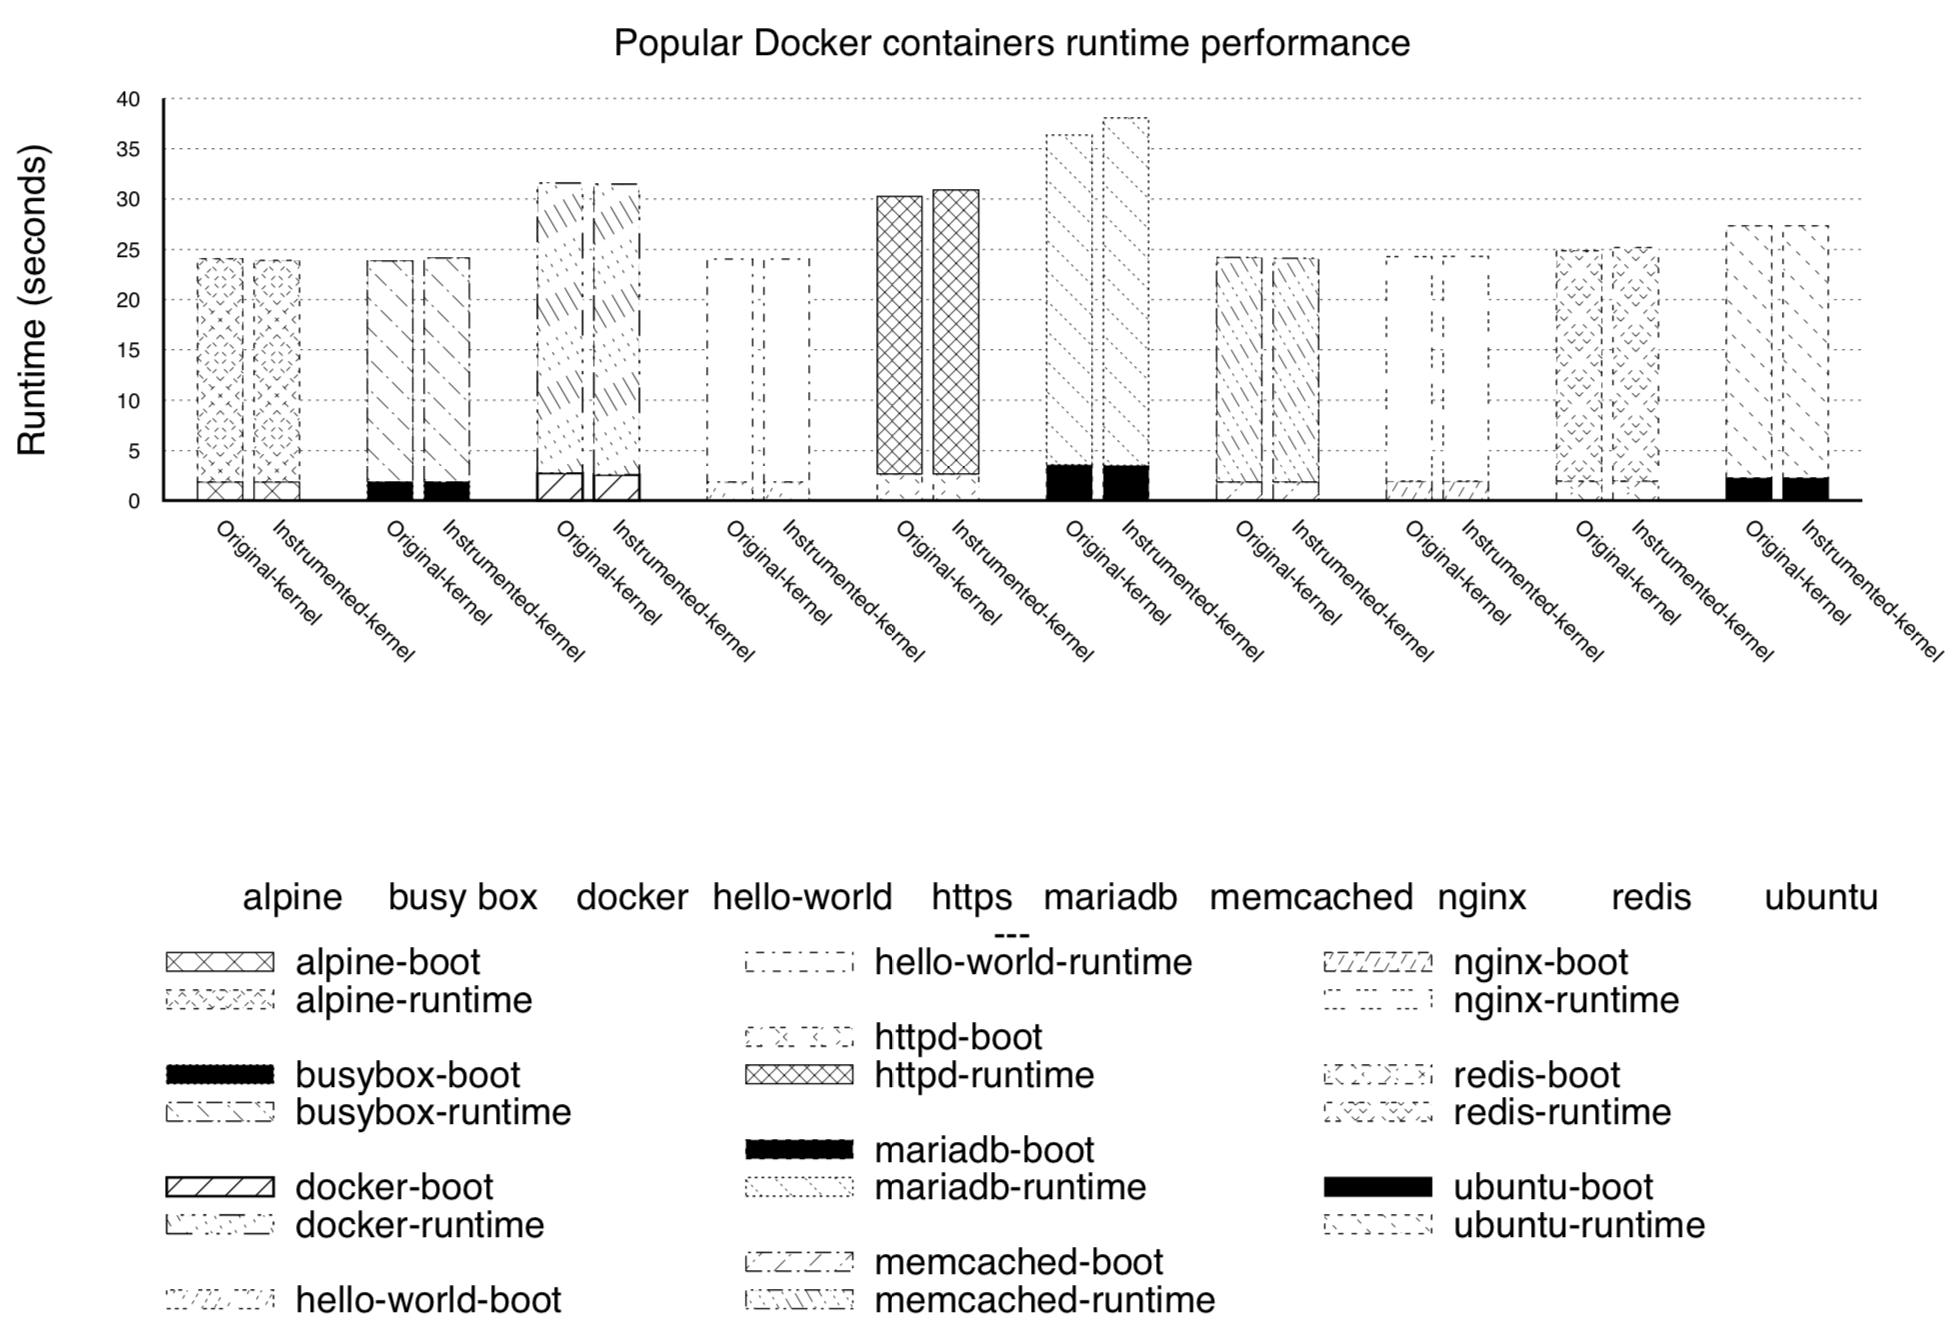
\includegraphics[width=1.5\columnwidth]{diagram/performance.png}
\caption{\small Runtime performance comparison for the top 10 containers}
\label{fig:performance}
\end{figure*}

The original Linux kernel image used for the LinuxKit test  is sized at 163,012,008 bytes. In comparison, UnPAK is sized at 163,622,440 bytes. 
Thus the extra memory space added by our modified kernel was only about 0.37\%. In addition, for both runtime and memory space UnPAK has negligible overhead.

\subsection{Comparison with existing kernel tailoring approaches}
\label{sec.evaluation.5} 
Lastly, we needed to compare our kernel tailoring approach with similar strategies dedicated to eliminating  inefficient and unnecessary code that can lead to vulnerabilities. 
We selected three current kernel tailoring  strategies and examined how our popular paths metric stacked up in terms of flexibility of application, 
ability to reduce the size of the attack surface, and other security and functionality issues. To do so, we utilized both published data and results of replication tests on available datasets. 

\subsubsection{Goals and approaches of current strategies}
\label{sec.evaluation.5.1}
While all three works  propose kernel tailoring strategies similar in some ways to our own, the main goals  of these strategies and their implementations vary. 
We start by summarizing these similarities and differences, as shown in Table \ref{tab:existing-approaches}.  

\begin{table}
\begin{center}
\caption{Existing Kernel Tailoring Approaches}
\label{tab:existing-approaches}
\begin{tabular}{l|l|l}
 Work & Main Goals & Main Approach \\
 \hline
 UnPAK & Reduce the kernel & Dynamic analysis \\
  (this paper) &  attack surface & / profiling + \\
  & for a container application & source code modification \\
 \hline
 Alharhi et al. & Reduce the number of & Tailoring the kernel \\
 \cite{SALAD18} & reported kernel CVE bugs & configuration based on \\
 & & vulnerability \\ 
 & & dependencies \\
 \hline
 Kurmus et al. & Reduce the kernel & Kernel automatically \\
 \cite{NDSS13} & attack surface for & configured  based on \\
 & a given user program & specific user \\
 & & application workloads \\
 \hline
 Kang et al. & Reduce the kernel & Automatic kernel \\
 \cite{Linux-Kernel-Tailoring-Framework} & attack surface &  configuration based on \\
 & & profiling and fixing \\
 & & configs for boot
\end{tabular}
\end{center}
\end{table}

The work of Alharhi et al. \cite{SALAD18} seeks to improve security by eliminating a selected group of reported CVE kernel bugs. 
Using a static-analysis strategy, this research team aims to establish a dependency between the CVE kernel bugs and particular kernel configuration options. 
Based on these dependencies, they were able to tailor the kernel to reduce the number of CVE bugs exposed . 
The key difference between their approach and the work presented in this paper is that Alharhi et al. explicitly designed their kernel tailoring strategy to find existing CVE bugs. 
As such, its usefulness may expire as new bugs are added. One advantage of our approach is that it is effective in predicting future bugs. 
In fact, in the evaluation above (Section~{\ref{sec.evaluation.2}}), we have shown that the popular paths approach was able to help predict and avoid 94\% of the zero-day bugs reported after the metric was published \cite{Lock-in-Pop}. 

Alternatively, Kurmus et al. \cite{NDSS13}, and Kang et al. \cite{Linux-Kernel-Tailoring-Framework} both aimed to reduce the kernel attack surface, 
but utilized different techniques.  Kurmus et al. modified its kernel configuration by disabling certain options and thus removing unneeded code. 
The researchers used profiling and dynamic analysis to identify which options to disable. Later, Kang et al. \cite{Linux-Kernel-Tailoring-Framework}, 
also attempted to reduce the attack surface, while making the kernel perform with greater stability. Their work began with an existing tool called undertaker-tailor \cite{NDSS13}, 
which was not very stable and, in some cases, produced kernel images that could not boot or function properly. By fixing configuration options needed at the booting stage, 
their tool, called Linux Kernel Tailoring Framework \cite{Linux-Kernel-Tailoring-Framework}, was able to produce tailored kernels that were more consistently reliable. 
Both of these research strategies required a mapping between the profiled kernel footprint and the kernel configuration, and the kernel was tailored through configuration options. 
In contrast, the kernel code tailoring in the popular paths related work was directly based on the data gathered from the popular paths.

\subsubsection{How do the tailored kernels compare by percent of tailoring and reduction of attack surface?}
\label{sec.evaluation.5.2}
We studied each of the current kernel tailoring approaches described above, and compared them with our work. 
Specifically, we utilized two criteria in our comparison: how much code in the kernel was tailored (modified) in each case, 
and how much of the attack surface could be reduced (as shown in Table \ref{tab:tailored-kernels}). For the  Linux Kernel Tailoring Framework \cite{Linux-Kernel-Tailoring-Framework}, 
we were able to access the data from their open source online repository \cite{Linux-Kernel-Tailoring-Framework} and so we ran the code and workload on our lab machine. 
The numbers used for the other initiatives were obtained from their conference presentations \cite{NDSS13}. 

The comparison shows that all tools were able to tailor the kernel code by 50\% or more, except in certain instances in Alharhi’s  \cite{SALAD18} results. 
UnPAK tailored the largest percentage number of  all four tools at 80\% of the kernel code. 
Furthermore, UnPAK achieved the largest reduction in attack surface. 
From a security standpoint, this is a more important and urgent factor than the code size reduction, as it means fewer chances for attackers to exploit zero-day vulnerabilities. 

\begin{table}
\caption{Comparison of the Tailored Kernels}
\label{tab:tailored-kernels}
\begin{tabular}{l|l|l}
 Work & Code tailored & Attack surface reduction \\
  & by size (percent) & (percent) \\
 \hline
 UnPAK & 80\% & 94\% \\
 \hline
 Alharhi et al. \cite{SALAD18} & 34\%-74\% & 89\% \\ 
 \hline 
 Kurmus et al. \cite{NDSS13} & 50\% & 50\%-85\% \\ 
 \hline
 Kang et al. \cite{Linux-Kernel-Tailoring-Framework} & 78\% & N/A
\end{tabular}
\end{table}

\begin{table*}
\caption{Limitations Comparison}
\label{tab:limitations}
\begin{tabular}{l|l|l|l|l}
 Work & Coarse-grained & Kernel trace not generic & Not bootable or working stably & Runtime performance overhead \\
 \hline
 UnPAK & \color{red}{\ding{55}} & \color{red}{\ding{55}} & \color{red}{\ding{55}} & \color{red}{\ding{55}} \\
 & & & & negligible overhead \\ 
 & & & & (0.1\% runtime; 0.37\% memory \\ 
 & & & & in its current configuration) \\
 \hline
 Alharhi et al. \cite{SALAD18} & \color{blue}{\ding{51}} & \color{blue}{\ding{51}} & \color{red}{\ding{55}} & N/A \\ 
 \hline 
 Kurmus et al. \cite{NDSS13} & \color{blue}{\ding{51}} & \color{blue}{\ding{51}} & \color{blue}{\ding{51}} (not stable) & \color{red}{\ding{55}} (no overhead) \\ 
 \hline
 Kang et al. \cite{Linux-Kernel-Tailoring-Framework} & \color{blue}{\ding{51}} & \color{blue}{\ding{51}} & \color{red}{\ding{55}} & \color{red}{\ding{55}} no overhead, \\ 
 & & & & and a little better than \\ 
 & & & & the original kernel in some cases \\
\end{tabular}
\color{blue}{\ding{51}: has this limitation;}
\color{red}{\ding{55}: does not have this limitation}
\end{table*}

\subsubsection{Are there differences in limitations?}
\label{sec.evaluation.5.3}
In practice, there may be conditions that prevent a tailored kernel from being useful. 
We extracted a few identified limitations in the past strategy examples to see if UnPAK would also be vulnerable to these conditions.  
The limitations are: 
\begin{itemize}
	\item \textbf{Coarse-grained tracing:} Some approaches only work at the function, file, or library level, which, as discussed in Section~{\ref{sec.evaluation.2}}, offer less flexibility in how a kernel can be tailored. This limitation could result in some user applications not being supported, or in missing opportunities for further code reduction that could be done at a finer level. 
	\item \textbf{Kernel trace is not generic:} An approach that only works for specific target applications could seriously affect the usefulness of the tool. 
	\item \textbf{Kernel is not bootable or able to work in a stable manner:} Some approaches may result in an unstable kernel that is not able to boot or function correctly every time. This will severely limit its usage. 
	\item \textbf{Large runtime performance overheads:} If the runtime overhead is too large, users are less likely to use the strategy, even if it can effectively reduce attack surfaces .   
\end{itemize}

Through this comparison (Table \ref{tab:limitations}), UnPAK suffers the least number of limitations, and is thus a more practical solution. 

Kernel tailoring strategies are important tools to improve system security. Through the comparison of UnPAK and three other strategies, 
we found that the popular-paths based approach was able to achieve the largest reduction in the kernel attack surface with little overhead in runtime performance 
and memory usage in its current configuration. Perhaps more importantly, it is a strategy that is not tied to a specific application or use case. 
Therefore, we believe that the UnPAK approach provides a more general and practical container security solution to users and developers. 
to secure the running environment of their container applications. 